% !TeX root = ../artigo.tex
\section{CLIENTE OPENLDAP}

Com o servidor finalizado, as contas e grupos de usuários já puderam ser criadas e armazenadas no diretório LDAP, com isso restou apenas as configurações adequadas em cada máquina, para fazer com que estas fossem capazes de ler, tanto os usuários para fins de autenticação, quanto os grupos criados para definição de permissões.

Como as máquinas existentes no PET Computação IFTM Campus Ituiutaba, possuíam mais de um sistema operacional, foi necessário criar opções de configuração para sistemas Unix, e Windows.

Além disso é importante ressaltar, que como dito antes, o OpenLDAP foi criado para ser uma ferramenta exclusiva de ambientes Linux, por mais que ele possa ser adaptado para funcionar no Windows, ele ainda não é capaz de oferecer todas as suas funcionalidades a este sistema.

\subsection{INSTALAÇÃO NO AMBIENTE UNIX}

Para a configuração do cliente Unix, foi usado o Arch Linux como sistema operacional, as configurações em sistemas Unix são muito semelhantes, porém em distribuições distintas pode ser que os passos utilizados podem ser diferentes dos aqui demonstrados.

\subsubsection{INSTALAÇÃO E CONFIGURAÇÃO DO PACOTE OPENLDAP}

Inicialmente foi necessário por meio do comando abaixo, instalar pacotes relacionados ao LDAP e facilitar a integração do sistema com servidores deste protocolo.

\begin{lstlisting}
    sudo pacman -S openldap libldap nss-pam-ldapd open-ldap-clients
\end{lstlisting}

Os propósitos de cada pacote mencionado no comando são:
\begin{itemize}
    \item openldap: Este é o pacote principal que instala o servidor de diretórios OpenLDAP.
    \item libldap: Este pacote contém a biblioteca de cliente LDAP. Ele fornece APIs para aplicativos que desejam interagir com servidores LDAP.
    \item nss-pam-ldapd: Esse pacote fornece serviços de nomes e autenticação para integrar sistemas Linux com um servidor LDAP.
    \item open-ldap-clients: Este pacote instala utilitários de linha de comando para interagir com servidores LDAP, como o OpenLDAP.
\end{itemize}

Após os pacotes serem instalados, foi necessário configurar a forma como o cliente LDAP (no caso, o OpenLDAP) se conecta a um servidor LDAP. Isso pôde ser feito por meio das alterações adequadas do arquivo seguinte.

\begin{lstlisting}
    /etc/openldap/ldap.conf
    BASE            dc=example,dc=com
    URI             ldap://localhost
\end{lstlisting}

Essas configurações são essenciais para definir o ponto base e o servidor LDAP ao qual o cliente se conectará. No entanto, essas configurações são específicas do ambiente e devem ser ajustadas para corresponder a configuração LDAP estabelecida.

\subsubsection{CONFIGURAÇÕES DE AUTENTICAÇÃO LDAP}

Na instalação dos pacotes, realizada na seção anterior, o pacote \textit{nss-pam-ldapd} foi instalado para habilitar a integração com servidores LDAP. 

Além disso, o arquivo \verb|/etc/nsswitch.conf|, que desempenha um papel central na configuração do NSS (Name Service Switch), um recurso do sistema que gerencia várias fontes de informações, foi editado. Este arquivo instrui o NSS sobre quais fontes de dados devem ser usadas para quais bancos de dados do sistema.

Foi necessário adicionar a diretiva 'ldap' aos bancos de dados apropriados. Portanto, o arquivo \verb|/etc/nsswitch.conf| foi configurado da seguinte maneira:

\begin{lstlisting}
    /etc/nsswitch.conf
    passwd: files `\textbf{ldap}`
    group: files `\textbf{ldap}`
    shadow: files `\textbf{ldap}`
\end{lstlisting}

Essas configurações permitiram a integração bem-sucedida do sistema com fontes de dados LDAP, possibilitando ver os usuários cadastrados no servidor ao executar o comando \textbf{getent passwd} no cliente.

Na configuração do PAM (Pluggable Authentication Module), a primeira edição foi feita no arquivo \verb|/etc/pam.d/system-auth|. Este arquivo é incluído na maioria dos outros arquivos do diretório /etc/pam.d, o que significa que as alterações feitas aqui se propagarão para várias partes do sistema. No entanto, é importante observar que atualizações no pacote PAM base podem afetar esse arquivo \cite{archlinux}.

Foi adicionado o termo 'pam\_ldap.so', marcado como 'sufficient' no topo de cada seção, exceto na sessão 'session', cuja alteração é opcional. As configurações realizadas definem as políticas de autenticação e controle de contas.

\begin{lstlisting}
    /etc/pam.d/system-auth
    `\textbf{auth}`      `\textbf{sufficient pam\_ldap.so}`
    auth      required  pam_unix.so     try_first_pass nullok
    auth      optional  pam_permit.so
    auth      required  pam_env.so
    
    `\textbf{account}`   `\textbf{sufficient pam\_ldap.so}`
    account   required  pam_unix.so
    account   optional  pam_permit.so
    account   required  pam_time.so
    
    `\textbf{password}`  `\textbf{sufficient pam\_ldap.so}`
    password  required  pam_unix.so     try_first_pass nullok sha512 shadow
    password  optional  pam_permit.so
    
    session   required  pam_limits.so
    session   required  pam_unix.so
    `\textbf{session}`   `\textbf{optional  pam\_ldap.so}`
    session   optional  pam_permit.so
\end{lstlisting}

Além disso, é importante mencionar a configuração do arquivo \verb|/etc/pam.d/su| . Neste arquivo, o termo 'pam\_ldap.so' é incluído como 'sufficient', permitindo que a autenticação do usuário seja verificada com sucesso no diretório LDAP. A adição de 'use\_first\_pass' na seção de autenticação do módulo 'pam\_unix.so' indica que a senha deve ser passada para o módulo em vez de solicitar novamente ao usuário.

\begin{lstlisting}
    /etc/pam.d/su
    auth      sufficient    pam_rootok.so
    `\textbf{auth}`      `\textbf{sufficient    pam\_ldap.so}`
    auth      required	pam_unix.so `\textbf{use\_first\_pass}`
    `\textbf{account}`   `\textbf{sufficient    pam\_ldap.so}`
    account   required	pam_unix.so
    `\textbf{session}`   `\textbf{sufficient    pam\_ldap.so}`
    session   required	pam_unix.so
\end{lstlisting}

Para permitir que os usuários editem suas senhas, o arquivo \verb|/etc/pam.d/passwd| também foi configurado, com 'pam\_ldap.so' incluído como 'sufficient'. Isso permite que as senhas sejam atualizadas no diretório LDAP quando os usuários as modificam.

\begin{lstlisting}
    /etc/pam.d/passwd
    `\textbf{password}`        `\textbf{sufficient      pam\_ldap.so}`
    password        required        pam_unix.so sha512 shadow nullok
\end{lstlisting}

Para fazer a criação de pastas pessoais ao fazer login, foi adicionado o termo 'pam\_mkhomedir.so' à seção 'session' do arquivo \verb|/etc/pam.d/system-login|, colocado acima das diretivas 'sufficient'. Essa modificação é responsável por ativar a criação de pastas pessoais ao fazer login por meio de um tty, SSH, xdm, sddm, gdm, etc \cite{archlinux}. 

Além disso foi aplicada uma mudança semelhante ao arquivo do PAM, \verb|/etc/pam.d/su-l|, para habilitar esse comportamento na sessão de 'su --login'.

\begin{lstlisting}
    /etc/pam.d/system-login 
    session    optional   pam_loginuid.so
    session    include    system-auth
    session    optional   pam_motd.so          motd=/etc/motd
    session    optional   pam_mail.so          dir=/var/spool/mail standard quiet
    -session   optional   pam_systemd.so
    session    required   pam_env.so
    `\textbf{session}`    `\textbf{required}`   `\textbf{pam\_mkhomedir.so skel=/etc/skel umask=0077}`
    
    /etc/pam.d/su-l
    `\textbf{session}`    `\textbf{required        pam\_mkhomedir.so skel=/etc/skel umask=0077}`
    session    sufficient      pam_ldap.so
    session    required        pam_unix.so
\end{lstlisting}

Por fim, para permitir o uso do 'sudo', que concede privilégios administrativos temporários, por usuários do LDAP, foi modificada a configuração do PAM no arquivo \verb|/etc/pam.d/sudo|, adicionando o termo 'pam\_ldap.so' para indicar que a autenticação pelo LDAP é aceitável para os privilégios.

\begin{lstlisting}
    /etc/pam.d/sudo
    `\textbf{auth}`      `\textbf{sufficient    pam\_ldap.so}`
    auth      required      pam_unix.so  `\textbf{try\_first\_pass}`
    auth      required      pam_nologin.so
\end{lstlisting}

Além da configuração do PAM, foi incluído no arquivo \verb|/etc/openldap/ldap.conf|, o grupo existente no servidor LDAP, contendo os usuários destinados a possuírem privilégios, de acordo com as configurações recomendadas abaixo.

\begin{lstlisting}
    /etc/openldap/ldap.conf
    sudoers_base ou=sudoers,dc=example,dc=org
\end{lstlisting}

\subsection{INSTALAÇÃO NO AMBIENTE WINDOWS}

Para a instalação do cliente no ambiente Windows, foi instalado o software 'pGina' na versão 3.1.8, o pGina é uma alternativa ao provedor de credenciais padrão do Windows, que é a parte do sistema responsável por gerenciar os logins. Usando plug-ins, o pGina possibilita a configuração de vários aspectos do processo de login, abrangendo desde a autenticação e autorização até o registro de eventos e a manipulação de terminais  \cite{pginauser}.

\begin{figure}[h]
	\centering
	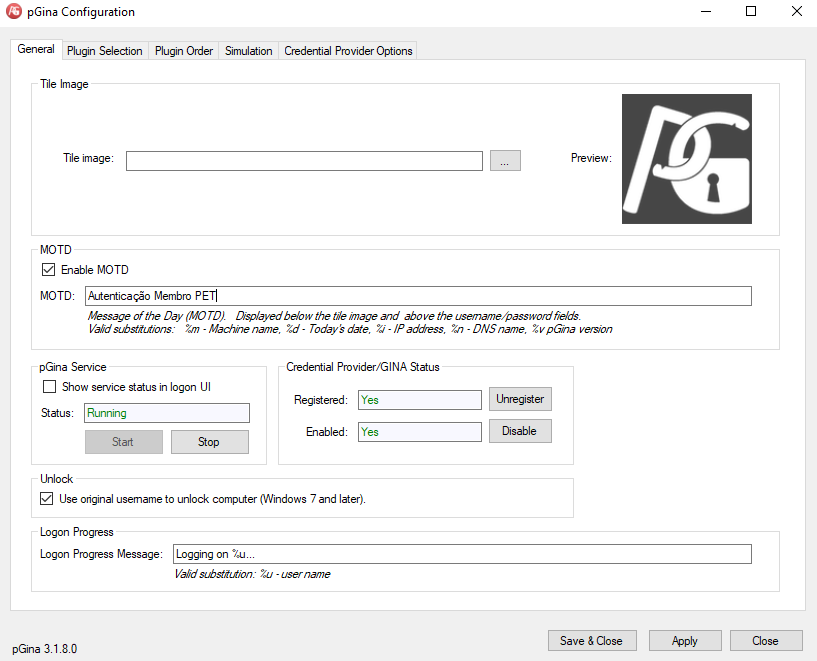
\includegraphics[scale=0.5]{textuais/PGina.png}
	\caption{Software de configuração do pGina
	\label{fig:pgina1}}
\end{figure}

O pGina administra o processo de login no Windows por meio da delegação de tarefas a um conjunto de plugins, que podem ser zero ou mais. Esses plugins têm a responsabilidade de determinar se o usuário é realmente quem alega ser (autenticação), decidir se o usuário deve ter acesso (autorização) e executar outras ações relacionadas ao login.

Para a configuração, foram adicionadas as três etapas do plugin 'LDAP': a 'Autenticação', a 'Autorização' e o 'Gateway'. Também foi alterada a ordem de leitura dos plugins existentes, dando prioridade ao 'LDAP', 

\begin{figure}[ht]
    \begin{subfigure}{0.48\textwidth}
    	\centering
    	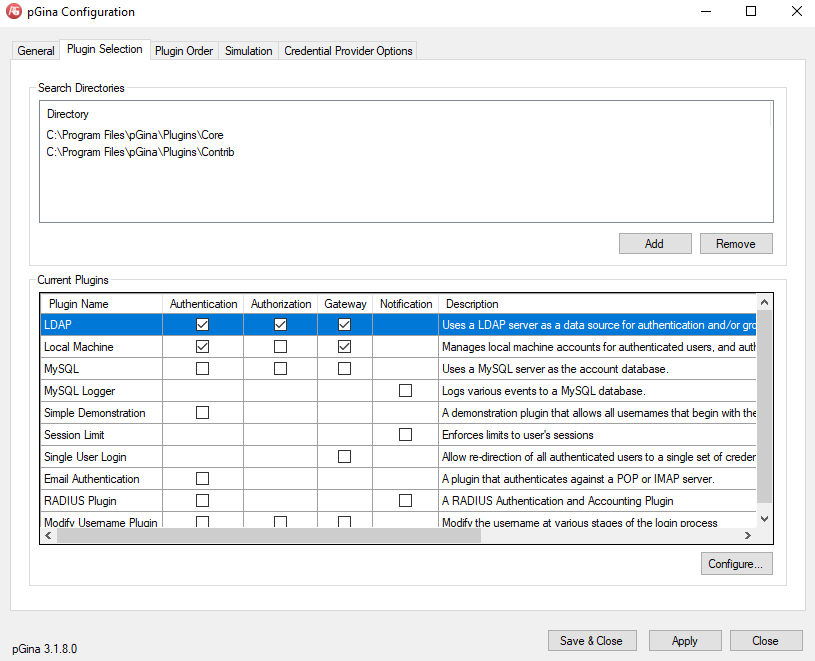
\includegraphics[width=\linewidth]{textuais/PGina2.png}
    	\caption{Seleção dos plugins
    	\label{fig:pgina2}}
    \end{subfigure}%
    \hspace{0.04\textwidth} % Espaço horizontal
    \begin{subfigure}{0.48\textwidth}
    	\centering
    	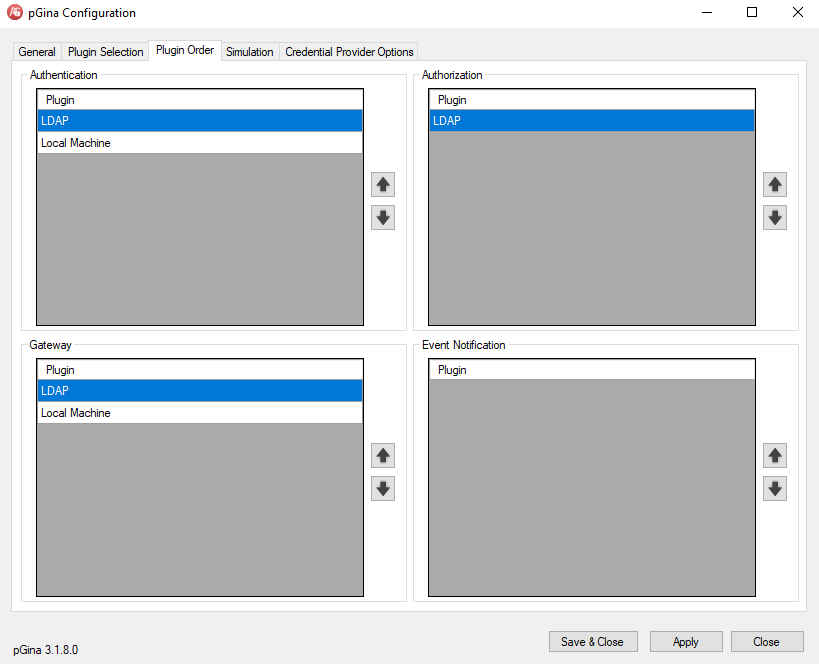
\includegraphics[width=\linewidth]{textuais/PGina3.png}
    	\caption{Ordem de leitura dos plugins
    	\label{fig:pgina3}}
    \end{subfigure}
    \caption{Configuração dos plugins do pGina}
    \label{fig:figuras}
\end{figure}

O plugin de autenticação LDAP fornece serviços de autenticação através de um servidor LDAP. Ele mapeia o nome de usuário para um Nome Distinto (DN) LDAP e tenta vincular-se ao servidor LDAP usando o DN. Se a ligação for bem-sucedida, ela fornecerá um resultado positivo ao serviço pGina \cite{pginaldap}.

Nas configurações do plugin, foram adicionados à seção do LDAP Server: o host, a porta, o DN 'admin', a senha, e o endereço para acessar os grupos, todos adequados ao servidor LDAP criado anteriormente, como será demonstrado na figura \ref{fig:pgina4}.

Na seção de 'Autenticação', foi indicado ao plugin para procurar pela DN do usuário no momento da autenticação, procurando pelo 'uid' correspondente no servidor LDAP, caso exista.

Por fim na seção de 'Gateway', foi adicionada a regra que caso o usuário correspondente, seja pertencente do grupo 'Adiminstrator', existente no servidor LDAP, ele será automaticamente movido ao grupo local 'Administradores' do Windows, que fornece ao usuário os privilégios de admin no sistema. 

\begin{figure}[ht]
    \begin{subfigure}{0.48\textwidth}
    	\centering
    	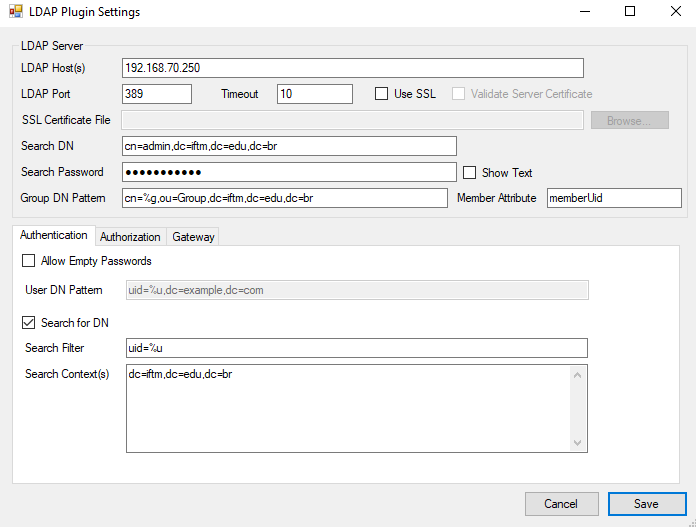
\includegraphics[width=\linewidth]{textuais/PGina4.png}
    	\caption{Autenticação
    	\label{fig:pgina4}}
    \end{subfigure}%
    \hspace{0.04\textwidth} % Espaço horizontal
    \begin{subfigure}{0.48\textwidth}
    	\centering
    	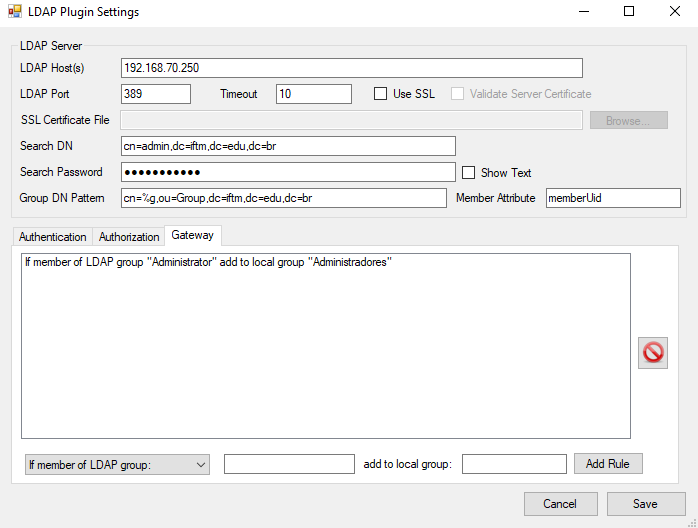
\includegraphics[width=\linewidth]{textuais/PGina5.png}
    	\caption{Gateway
    	\label{fig:pGina5}}
    \end{subfigure}
    \caption{Configuração do plugin LDAP}
    \label{fig:figuras}
\end{figure}